\documentclass{article}
  % M�rgenes
  \textheight    = 20cm
  \textwidth     = 18cm
  \topmargin     = -2cm
  \oddsidemargin = -1cm
  % Sangr�a
  \parindent     =  0mm
  %Paquetes 
  %  deben venir con la distribuci�n TeX 
  %  o se pueden poner en la misma carpeta de este archivo .tex
  \usepackage{amsmath, amssymb, amsfonts, latexsym}
  \usepackage[T1]{fontenc}
  \usepackage[latin1]{inputenc}
  \usepackage{graphicx}
  \usepackage{pstricks}
  \title{Diseinua}
  \author{Ieltzu Irazu, Mikel de Velasco, Jorge Nieto}
  \date{29 de enero de 2010}

  %Inicio del cuerpo del documento
\begin{document}
\newpage
\maketitle
\begin{center}
	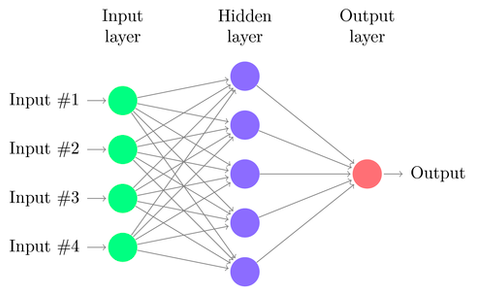
\includegraphics[width=10cm]{img/portada.png} 
\end{center}
\newpage
\section{Azaleko Orria / Aurkibidea}
\begin{enumerate}
	\item {\sc Azaleko Orria / Aurkibidea\dotfill 2}
	\item {\sc Aurkezpena\dotfill 3}
	\item {\sc Klaseen diseinua\dotfill 3}
\end{enumerate}
\newpage
\section{Aurkezpena}
Dokumentu honen bidez, 	
Multilayer Perceptron eta Naive Bayes eredu igarleak konparatzen ditu.
\section{Klaseen diseinua}
Proiektua hiru atal nagusitan banandu dugu. Lehenengoan, datuak aurreprozezatzen dira, bigarrenean, eredua aterako da eta azkenik instantzia berriak ebaluatzeko jarriko da.
\begin{enumerate}
	\item \textbf{Aurreprozezamendua} \\
		Atal honetan, bereiziki ``R-weka.filters.unsupervised.attribute.Obfuscate'' relation-a duten arff fitxategiekin (praktika honetan lan egin behar zirenak) lan egingo dugu. Horregatik behean aipatzen diren filtroak praktika honekin lan egiteko daude. \\
		Aurre prozezamenduan hurrengo klase eta metodoak erabiliko dira.
		\begin{enumerate}
			\item {\bf Aurreprozezadorea:}\\
			Klase hau, {\red Preprocess.jar} exekutagarriak egikarituko duen lehenengo klasea izango da, beraz klase nagusia izango da.\\
			Bere metodoa hurrengoa da:
			\begin{itemize}
				\item {\bf main}\\
				``main'' metodoan, argumentu bezala konsolatik {\blue train.arff} eta {\blue dev.arff} fitxategiak pasatuko dizkiogu, eta nahi izanez gero (instantzia asko badira) 0-100 arteko zenbaki bat pasatu ahal izango diogu, zenbaki honek instantzia kopuru gutxiagorekin lan egiteko izango da (adb: 70 pasatzen badiogu instantzien \%70-rekin lan egingo dugu).\\
				Klase honetan metodo bakarra egotea erabaki dugu. Wekak dituen liburutegiak filtroen klseak dituztelako eta `main' metodo honetan, filtro guztiak aplikatuko ditugu:
				\begin{enumerate}
					\item {\bf Discretize:}\\
					An instance filter that discretizes a range of numeric attributes in the dataset into nominal attributes.
					\item {\bf InterquartileRange:}\\
					A filter for detecting outliers and extreme values based on interquartile ranges.
					\item {\bf Randomize:}\\
					Randomly shuffles the order of instances passed through it. The random number generator is reset with the seed value whenever a new set of instances is passed in.
					\item {\bf RemoveUseless:}\\
					This filter removes attributes that do not vary at all or that vary too much. All constant attributes are deleted automatically, along with any that exceed the maximum percentage of variance parameter. The maximum variance test is only applied to nominal attributes.
					\item {\bf RemoveWithValues:}\\
					Filters instances according to the value of an attribute.
					\item {\bf AttributeSelection:}\\
					A supervised attribute filter that can be used to select attributes. It is very flexible and allows various search and evaluation methods to be combined.
				\end{enumerate}
				`Discretize', `Radomize' eta `RemoveUseless' ``multifilter'' batean sartzen dira batera egiteko. `InterquartileRange' aplikatu ostean bi atributu sortzen ditu, atributu hoiekin `outlier' instantziak eta `extreme values' kenduko dira `RemoveWithValues' eta `Remove' metodoekin. \\
				Filtro guztiak aplikatu hondoren sortutako instantzia berriak fitxategi batera pasatzen dira, geroago berrerabiltzeko.
			\end{itemize}
		\end{enumerate}
		
	\item \textbf{Modeloa egitea} \\
		Atal honetan, entrenamendu multzoak jasoko dira ({\blue trainaurre.arff} eta {\blue devaurre.arff}), `Baseline'-aren (`OneR') eta `MultilayerPerceptron' aldagaien ekorketa egingo da, geroago bien inferentzia (ez zintzoa, HoldOut (70 / 30), HoldOut ({\magenta train} eta {\magenta dev}) eta 10FoldCrossValidation), azkenik bien modeloak gordeko dira fitxategi batean.\\
		Modeloak hurrengo klase eta metodoak erabiliko ditu.
		\begin{enumerate}
			\item {\bf Modeloa:}\\
			Klase hau, {\red GetModel.jar} exekutagarriak egikarituko duen lehenengo klasea izango da, beraz klase nagusia izango da.\\
			Bere metodoa hurrengoa da:
			\begin{itemize}
				\item {\bf main}\\
				``main'' metodoan, argumentu bezala konsolatik {\blue trainaurre.arff} eta {\blue devaurre.arff} fitxategiak pasatuko dizkiogu. Fitxategi hauek pasatu behar zaie orden horretan. Horren ondoren ({\magenta trainaurre} instantzien artean klase minoritarioa aterako da. Hori egin eta gero, {\magenta trainaurre} eta {\magenta devaurre} instantziak {\magenta trainetadev} instantzia multzo bakarrean batuko dira. Eta beste aldaera batzuk kalkulatuko dira:
				\begin{itemize}
					\item {\magenta trainetadev70} multzoa: {\magenta trainetadev} multzoaren instantzien \%70 barruan dituelarik.
					\item {\magenta trainetadev30} multzoa: {\magenta trainetadev} multzoaren instantzien \%30 barruan dituelarik.
				\end{itemize}
				Orain `Baseline' eta `MultilayerPerceptron' modeloekin hainbat ekintza egingo ditugu:
				\begin{enumerate}
\item Parametro ekorketa:\\ Klase minoritarioarekiko `weigthedMeasure'.
\begin{itemize}
\item Baseline:
\begin{itemize}
\item MinBucketSize
\item doNotCheckCapabilities
\end{itemize}
\item multilayerPerceptron:
\begin{itemize}
\item hiddenLayers
\item training Time
\end{itemize}

\end{itemize}

\item Bilaketa ez-exhaustiboa
\item Inferentzia
\begin{enumerate}
\item Ez-Zintzoa
\item HoldOut 70-30
\item HoldOut {\magenta train} eta {\magenta dev}
\item 10FoldCrossValidation
\end{enumerate}
Metodo bakoitzarekin fitxategi bat idatziko da  {\bf Idazlea} klasearekin eta {\bf fitxategiaEginOneR} eta {\bf fitxategiaEginMultilayerPerceptron} metodoekin hurrenez hurren ({\blue evaluationBaseline.txt} eta {\blue evaluationMultilayerPerceptron.txt}).
\end{enumerate}
Hau guztia egin eta gero modelak idatziko dira {\bf Idazlea} klasearekin eta {\bf modeloaIdatzi} metodoarekin.
\item {\bf minorityClassIndex:}\\
Metodo honek instantzia multzo bat jasotzen du eta klase minoritarioaren indezea ateratzen du.
			\end{itemize} 
		\end{enumerate}
\item \textbf{Sailkatzea}\\
Sailkatu behar diren instantzia multzo bat jasoko da eta fitxategi berri batean sailkatuko ditu.
\begin{enumerate}
\item {\bf Sailkatzailea}\\
Klase hau, {\red Classify.jar} exekutagarriak egikarituko duen lehenengo klasea izango da, beraz klase nagusia izango da.\\
Bere metodoa hurrengoa da:
\begin{itemize}
\item {\bf main:}\\
{\gray modeloaPath}, {\gray testPath} eta {\gray resultPath} jasotzen dira eta {\bf Irakutzailea} klaseak daukan {\bf modeloaKargatu} eta {\bf instantziakIrakurri} metodoekin {\magenta modeloa} eta {\magenta instantziak} kargatuko dira.\\
Horren oztean, {\magenta instantzia} guztiak klasifikatuko dira eta emaitza {\bf Idazle} klasearekin eta {\bf idatziInstantzia} metodoarekin {\gray resultPath} helbidean gordeko da.
\end{itemize}
\end{enumerate}
\item \textbf{Laguntzaile batzuk:}\\
Atal honetan, gure helburua betetzeko laguntzen diguten  beste bi klase azalduko da.Bi klase hauek {\bf Idazlea} eta {\bf Irakurtzailea} izena dute eta bere izena esaten duten bezala irakurtzeko eta idazteko balioko digute\\
		Laguntzaile klaseetan metodo hauek erabiliko dira.
		\begin{enumerate}
			\item {\bf Irakurtzailea:}\\
			Klase hau, irakurtzeko erabiliko dugun klasea da. Bai fitxategiak, bai modeloak irakurriko ditu.\\
			Bere metodoak hurrengoak dira:
			\begin{itemize}
				\item {\bf Irakurtzailea:}\\
					Klase honetako eraikitzailea da eta eraikitzaile guztiak bezala klasea eraikitzeko balio du.
				\item {\bf getIrakurtzailea:}\\
					Instantzia bakarra nahi dugunez EMA bat sortuko dugu eta beraz metodo honek instantzia bakarra izateko balio du.
				\item {\bf instantziakIrakurri:}\\
					Metodo honek irakurri nahi dugun fitxategiaren path-a jasoko da argumentu bezala. Metodoan jasotako fitxategi hori kargatuko da instantzia multzo batean eta bere atributuen artean zein den klasea zehaztuko da.
				\item {\bf modeloaKargatu:}\\
					Argumentu bezala kargatu nahi dugun modeloaren path-a jasoko da. Jasotako path horretatik modeloa kargatuko da.
			\end{itemize}
			\item {\bf Idazlea:}\\
			Klase hau, idazteko erabiliko dugun klasea da. Bai fitxategiak, bai modeloak idatziko ditu.\\
			Bere metodoak hurregoak dira:
			\begin{itemize}
				\item {\bf Idazlea:}\\
					Klase honetako eraikitzailea da eta eraikitzaile guztiak bezala klasea eraikitzeko balio du.
				\item {\bf getIdazlea:}\\
					Instantzia bakarra nahi dugunez EMA bat sortuko da eta beraz metodo honek instantzia bakarra izateko balio du.
				\item {\bf idatziInstantziak:}\\
					Argumentu bezala, instantzia multzo batzuk eta eraikiko den fitxategiaren path-a jasoko da. Metodoaren zehar jasotako patharekin fitxategi File bat eraikiko da. Jasotako instantziak, eraikitako fitxategian sartuko dira.
				\item {\bf fitxategiaEginOneR:}\\
					Metodo honetan haibat argumentu jasoko dira:
					\begin{itemize}
						\item {\bf path:}\\
							File bat eraikitzeko path-a izango da. 
						\item {\bf evaluator:}\\
							Metodoan erabilitako ebaluatzailea da.
						\item {\bf bMax:}\\
							Parametro ekorketan ateratako bucket size maximoa. 
						\item {\bf bucketSizeExhaustiboa:}\\
							Bucket size maximoa bilaketa ez exhaustiboan ateratakoa.
						\item {\bf estimazioMota:}\\
							One-R algoritmoaren estimatzailea jasoko da.
						\item {\bf berria:}\\
							Fitxategia berria izango denik ala ez zehaztuko da.
					\end{itemize}
					Parametro guzti horiek jasota fitxategi batean idatziko dira ebaluatuko diren parametro asko.
				\item {\bf fitxategiaEginMultilayerPerceptron:}\\
					Metodo honetan haibat argumentu jasoko dira:
					\begin{itemize}
						\item {\bf path:}\\
							File bat eraikitzeko path-a izango da. 
						\item {\bf evaluator:}\\
							Metodoan erabilitako ebaluatzailea da.
						\item {\bf estimador:}\\
							Multilayer Perceptronen estimatzailea jasoko da 
						\item {\bf hiddenLayersEzExhaustiboa:}\\
							Bucket size maximoa bilaketa ez exhaustiboan ateratakoa.
						\item {\bf estimazioMota:}\\
							Multilayer Perceptron algoritmoaren estimatzailea jasoko da.
						\item {\bf berria:}\\
							Fitxategia berria izango denik ala ez zehaztuko da.
					\end{itemize}
					Parametro guzti horiek jasota fitxategi batean idatziko dira ebaluatuko diren parametro asko.
				\item {\bf modeloaIdatzi:}\\
					Metodo honetan bi argumentu jasoko dira. Lehenengoa, modeloa idatzi nahi dugunaren path-a izango da. Bigarrena, erabili nahi den estimatzailea jasoko da. Metodo honetan, jasotako argumentuekin modeloa idatziko da. 
			\end{itemize}
		\end{enumerate} 
\end{enumerate}
\end{document}
